\chapter{Performance-Analyse der vorgegebenen Python-Implementierung}

\section{Komplexitätsanalyse}

\subsection{Speckle-Tracking}

Der erste Schritt des Speckle-Trackings ist, laut \citeauthor{Ber13, Coj17}, die Feststellung der starren Verschiebung \cite{Ber13, Coj17}. Werden hierfür feste Werte für diese angenommen, ist diese Komplexität konstant. Wird allerdings ein Korrelationsverfahren verwendet, so ist die Komplexität für die \gls{resolution} gleich $\mathcal{O}\left(\glssymbol{resolution} \cdot log\left(\glssymbol{resolution}\right)\right)$, da hierfür \glspl{FFT} eingesetzt werden können. 

Der nächste Verarbeitungsschritt ist der erste Durchlauf. Laut des Codes von \citeauthor{Coj17} werden hier die Eingabebilder zunächst durch die Selektion der \gls{ROI} auf die \glsfirst{rroi} \glssymbol{rroi} zugeschnitten und anschließend in quadratische Blöcke mit konstanter \gls{rblock} aufgeteilt \cite{Coj17}. Daraufhin werden die Blöcke aus den Bildern des ersten Sensors in den Gegenstücken des zweiten Sensors mittels des Template-Matchings gesucht. Liegt ein Block teilweise außerhalb der \gls{ROI}, so wird dieser, gemäß \citeauthor{Coj17}, hineinkorrigiert \cite{Coj17}. Der Durchlauf hat deshalb Komplexität: 

\begin{center}
	$\mathcal{O}\left(\frac{\gls{rroi} \cdot \gls{rblock} \cdot log\left(\gls{rblock}\right)}{\gls{rblock}}\right) = \mathcal{O}\left(\gls{rroi} \cdot log\left(\gls{rblock}\right)\right)$
\end{center}

Da die \gls{rblock} konstant und die Dauer der einzelnen Suchvorgänge somit ebenfalls als konstant angenommen werden können, liegt dieser Durchlauf in der linearen Komplexitätsklasse. Die anschließende Interpolation wird auf alle Pixel des Bildes angewandt und hat demzufolge eine Komplexität von $\mathcal{O}\left(\gls{rroi}\right)$. Im darauf folgenden zweiten Durchlauf werden Subbilder, wie in Abschnitt \ref{sec:speckle-tracking} beschrieben, generiert. Durch die \glsfirst{uap} \glssymbol{uap} wird \gls{rroi}, und damit auch die Komplexität dieses Teils, mit dem Faktor $\gls{uap}^2$ verringert. Die \glsfirst{corrsize} \glssymbol{corrsize} nimmt auf das Template-Matching Einfluss, dessen Komplexität dadurch bei $\mathcal{O}\left(\gls{corrsize} \cdot log\left(\gls{corrsize}\right)\right)$ liegt. Der Einfluss der \glsfirst{gridResol} \glssymbol{gridResol} ist, ähnlich zu \gls{uap}, eine Verringerung mit dem Faktor $\gls{gridResol}^2$. Die Gesamtkomplexität der Template-Matchings im zweiten Durchlauf liegt somit bei:

\begin{center}
	$\mathcal{O}\left(\frac{\gls{rroi} \cdot \gls{corrsize} \cdot log\left(\gls{corrsize}\right)}{\gls{uap}^2 \cdot \gls{gridResol}^2}\right)$
\end{center}

Für die auf den Template-Matching-Prozess folgende Subpixel-Interpolierung werden, wie im Code von \citeauthor{Coj17} implementiert, neun Pixel in der Umgebung des Maximums jeder Übereinstimmungsmatrix interpoliert \cite{Coj17}, womit dieser Schritt folgende Komplexität aufweist:

\begin{center}
	$\mathcal{O}\left(\frac{\gls{rroi}}{\gls{uap}^2 \cdot \gls{gridResol}^2}\right)$
\end{center}

Am Ende des Speckle-Tracking-Algorithmus wird versucht, nicht zuordenbare Ergebnisse mit einer anderen \glsfirst{corrsize} $\glssymbol{corrsize}'$ erneut zuzuordnen. Im schlimmsten Fall wird der zweite Durchlauf für die Hälfte der Subbilder \glssymbol{ncorr}-fach wiederholt, wobei \glssymbol{ncorr} die \gls{ncorr} repräsentiert. Bei höheren Fehlerraten über 50\% bricht das von \citeauthor{Coj17} entwickelte Programm ab \cite{Coj17}. In der hier als Grundlage vorliegenden Implementierung ist \gls{ncorr} gleich 6. Die Gesamtkomplexität des Speckle-Tracking-Algorithmus liegt damit in der Komplexitätsklasse:

\begin{center}
	$\mathcal{O}\left(\frac{\gls{rroi} \cdot \gls{corrsize} \cdot log\left(\gls{corrsize}\right) \cdot \gls{ncorr}}{\gls{uap}^2 \cdot \gls{gridResol}^2}\right)$
\end{center}

\subsection{Integration der Gradienten}

Um eine effiziente Integration der Gradienten zu ermöglichen, beruht der von \citeauthor{FC88} vorgeschlagene Algorithmus auf der Integration im Frequenzraum \cite{FC88}. Hierzu werden zuerst die Gradientenbilder mittels \glspl{FFT} in diesen Raum transformiert, dort in linearer Komplexität integriert und zum Schluss wieder zurücktransformiert. Aufgrund der Verwendung von \glspl{FFT} befindet sich dieser Algorithmus in der Komplexitätsklasse:

\begin{center}
	$\mathcal{O}\left(\gls{resolution} \cdot log\left(\gls{resolution}\right)\right)$
\end{center}

\subsection{Verarbeitungsroutine der Bilder}

Die Hauptroutine beginnt, gemäß \cite{Coj17}, mit einer trivialen Parameterinitialisierung, die als linear angenommen werden kann. Auf diese folgt die Hauptschleife, welche für die \gls{N_Paare} jeweils einmal ausgeführt wird \cite{Coj17}. Hierzu werden zuerst die Sensorbilder mittels der bei der Kalibrierung ermittelten Werte mit einer Komplexität von $\mathcal{O}\left(\gls{resolution}\right)$ korrigiert. Dem folgt, wie von \citeauthor{Coj17} implementiert, der Speckle-Tracking-Algorithmus und die Integration der Gradienten \cite{Coj17}. Die höchste Komplexität hat hier der Template-Matching-Algorithmus, welcher damit die Komplexitätsklasse der Hauptroutine festlegt auf:

\begin{center}
	$\mathcal{O}\left(\frac{\gls{N_Paare} \cdot\gls{rroi} \cdot \gls{corrsize} \cdot log\left(\gls{corrsize}\right) \cdot \gls{ncorr}}{\gls{uap}^2 \cdot \gls{gridResol}^2}\right)$
\end{center}

Diese Komplexitätsklasse liegt insbesondere für kleine \gls{ncorr}, \gls{uap} und \gls{gridResol} in der Oberklasse:

\begin{center}
	$\mathcal{O}\left(\gls{N_Paare} \cdot \gls{rroi} \cdot \gls{corrsize} \cdot log\left(\gls{corrsize}\right)\right)$
\end{center}

\section{Performance-Messungen}

\label{sec:performance-messungen}

\paragraph{Testsystem}

\begin{sloppypar}
Alle Benchmarks liefen auf der \textit{haswell}-Partition des Taurus-Supercomputers an der Technischen Universität Dresden. Jeder Knoten dieser Partition ist ausgestattet mit zwei Intel\textregistered \mbox{Xeon\textregistered} E5-2680 v3 \glspl{CPU}. Diese haben jeweils zwölf Rechenkerne, die mit bis zu 2.50 \gls{GHz} getaktet sind. HyperThreading war hierbei nicht aktiviert. Die Knoten haben 64 \gls{GiB} (\textit{haswell64}), 128 \gls{GiB} (\textit{haswell128}) oder 256 \gls{GiB} (\textit{haswell256}) Arbeitsspeicher zur Verfügung \cite{Mar17}. Zusätzlich ist pro Rechenknoten eine 128 \gls{GB} \gls{SSD} installiert. Es wurde unter anderem Python 2.7.11 mit numpy 1.10.1 und OpenCV 3.1.0 verwendet. Eine komplette Liste aller geladenen Module lässt sich auf dem GitHub-Repository dieses Projektes finden \cite{Sch18a}.
\end{sloppypar}

\paragraph{Konfigurationen}

Jede Konfiguration, bestehend aus Datensatz und Kernanzahl, wurde nach vier Aufwärmiterationen fünfmal ausgeführt. Hierbei wurden jeweils die reinen Ausführungszeiten des gesamten Skripts und einzelner Funktionen erfasst. Aus allen vorliegenden Zeiten wurden \gls{IO}-Zeiten herausgerechnet. Die Laufzeit mit den entsprechenden Datensätzen wurde auf unterschiedlich vielen Kernen von eins bis 24 gemessen. Jeder Benchmark lief exklusiv auf einem Knoten. 

Zur Leistungsfeststellung der vorliegenden Implementierung werden zwei verschiedene Arten von Datensätzen verwendet: \textit{Experiment 6} und \textit{Lenses}. Die \textit{Experiment 6}-Datensätze wurden hierbei von Ruxandra Cojocaru, Sébastien Bérujon und Eric Ziegler am 24. September und die \textit{Lenses}-Datensätze wurden von Thomas Roth, Raymond Barett, Sébastien Bérujon und Rafael Celeste am zehnten April 2017 an der Beamline BM05 der \gls{ESRF} aufgenommen \cite{CBZ17, RBB+17}. Die Bildpaare des \textit{Experiment 6}-Datensatzes wurden, wie in Abbildung \ref{fig:versuch} gezeigt, mit zwei Sensoren gleichzeitig aufgezeichnet, währenddessen die Bildpaare des \textit{Lenses}-Datensatzes aus Bildern ein und desselben Sensors stammen, wobei anfangs ein Bild als Referenz aufgenommen wurde. Die Eigenschaften dieser Typen werden in Tabelle \ref{tab:dataset_types} gegenüber gestellt. Die einzelnen Datensätze mit deren Anzahl der Bilder sind in Tabelle \ref{tab:datasets} zu finden. 

\begin{table}
	\begin{tabularx}{\textwidth}{@{} XXX @{}}
		\toprule
		& Experiment 6 & Lenses \\
		\hline
		\gls{rroi} & Sensor 1: $550px * 550px$ \newline
		Sensor 2: $1450px * 1450px$  & $1450px * 1550px$ \\
		\gls{gridResol} & 1 & 1 \\
		\gls{corrsize} & $91px * 91px$ & $41px * 41px$ \\
		\gls{uap} & 1 & 1 \\
		Pixelgröße & unterschiedlich & gleich \\
		\bottomrule
	\end{tabularx}
	\caption{Parameter der Datensatztypen gemäß \citeauthor{Coj17} \cite{Coj17}}
	\label{tab:dataset_types}
\end{table}

\begin{table}
	\begin{tabularx}{\textwidth}{@{} XXXXXXXX @{}}
		\toprule
		& \multicolumn{3}{c}{Experiment 6} & \multicolumn{4}{c}{Lenses} \\
		\cmidrule(lr){2-4}
		\cmidrule(lr){5-8}
		& Lenses 200 & Lenses 500 & Lenses 1500 & Set 1 & Set2 & \multicolumn{2}{X}{Set 3} \\
		\hline
		\gls{N_Paare} & 21 & 11 & 14 & 10 & 5 & 1 & 2 \\
		\bottomrule
	\end{tabularx}
	\caption{Anzahl der Bildpaare der Datensätze gemäß \citeauthor{Coj17} \cite{Coj17}}
	\label{tab:datasets}
\end{table}

\paragraph{Laufzeiten}

Die Laufzeiten der Konfigurationen, dargestellt in Abbildung \ref{fig:gesamtlaufzeiten}, variieren untereinander stark und reichen von ca. dreieinhalb Stunden für den \textit{Lenses Set 1}-Datensatz auf einem Kern bis hin zu ca. vier Minuten für den \textit{Lenses Set 3} Datensatz mit einem Bild auf 24 Kernen. Die Messpunkte sind hierbei dick hervorgehoben und die Skala ist logarithmisch eingeteilt. 

\begin{center}
	\begin{figure}[h!]
		\begin{subfigure}[b]{0.49\textwidth}
			\centering
			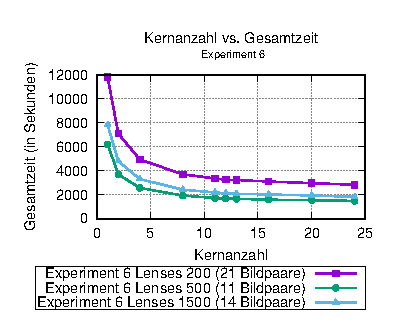
\includegraphics[width=\textwidth]{pdf/times_exp6}
			\caption[Experiment 6]{Experiment 6}
			\label{fig:times_exp6}
		\end{subfigure}
		\hfill
		\begin{subfigure}[b]{0.49\textwidth}
			\centering
			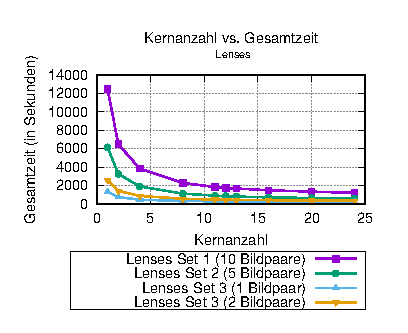
\includegraphics[width=\textwidth]{pdf/times_lenses}
			\caption[Lenses]{Lenses}
			\label{fig:times_lenses}
		\end{subfigure}
		\caption{Gesamtlaufzeiten}
		\label{fig:gesamtlaufzeiten}
	\end{figure}
\end{center}

Der Speed-Up des Programmes skaliert mit der Anzahl der Prozessorkerne nicht linear und flacht schnell ab. Der Speed-Up-Faktor für die \textit{Experiment 6}-Datensätze konvergiert gegen vier. Bei den \textit{Lenses}-Da\-ten\-sä\-tzen hingegen wird bei 24 Kernen ein Speed-Up von mehr als zehn erreicht. In den auf Abbildung \ref{fig:speedup} visualisierten Graphen ist eine starke Skalierung deutlich erkennbar. 

\begin{center}
	\begin{figure}[h!]
		\begin{subfigure}[b]{0.49\textwidth}
			\centering
			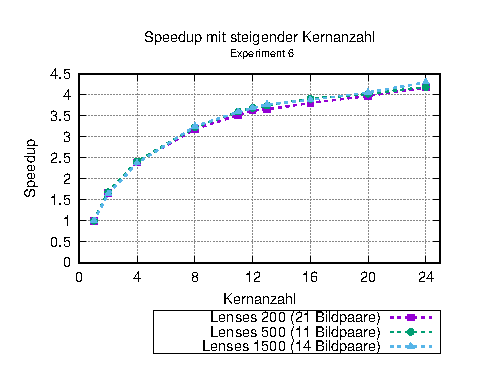
\includegraphics[width=\textwidth]{pdf/speedup_exp6}
			\caption{Experiment 6}
			\label{fig:speedup_exp6}
		\end{subfigure}
		\hfill
		\begin{subfigure}[b]{0.49\textwidth}
			\centering
			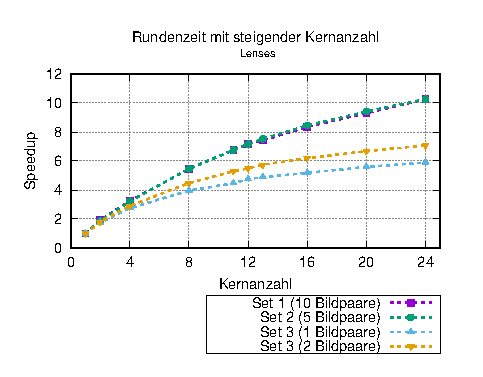
\includegraphics[width=\textwidth]{pdf/speedup_lenses}
			\caption{Lenses}
			\label{fig:speedup_lenses}
		\end{subfigure}
		\caption{Speed-Up}
		\label{fig:speedup}
	\end{figure}
\end{center}

Um Engpässe und besonders rechenaufwendige Funktionen zu identifizieren, wurde das Programm mit Zeitmessern versehen, die Ausführungszeiten und Aufrufanzahl protokolliert haben. Anschließend wurde es auf einem Rechenkern unter denselben Bedingungen, wie die anderen Konfigurationen, ausgeführt und die Zeiten wurden gemessen. Ein Überblick über das Gesamtprogramm mit seinen Subroutinen und deren Anteil an der Gesamtlaufzeit ist in Abbildung \ref{fig:perc_main} zu sehen.

\begin{center}
	\begin{figure}[h!]
		\begin{subfigure}[b]{0.5\textwidth}
			\centering
			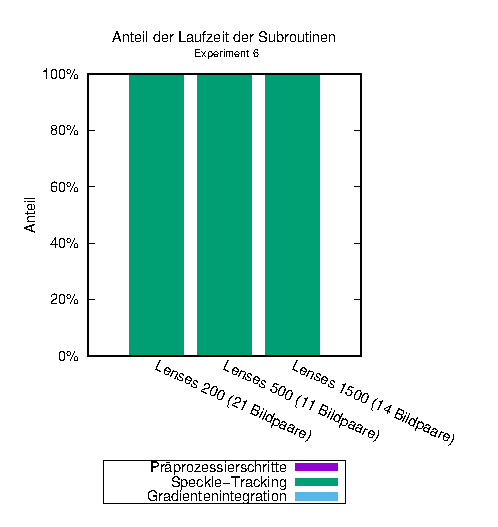
\includegraphics[width=\textwidth]{pdf/main_exp6}
			\caption{Experiment 6}
			\label{fig:perc_main_exp6}
		\end{subfigure}
		\begin{subfigure}[b]{0.5\textwidth}
			\centering
			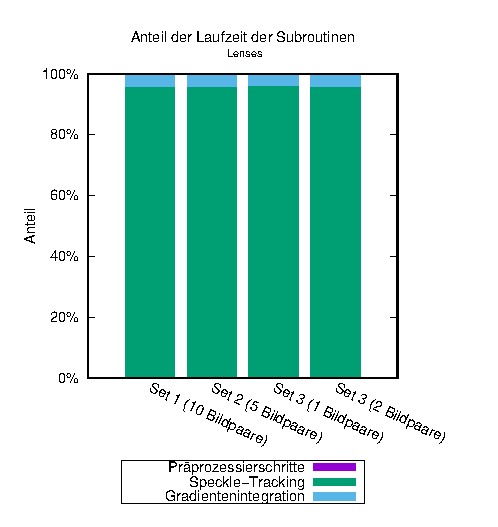
\includegraphics[width=\textwidth]{pdf/main_lenses}
			\caption{Lenses}
			\label{fig:perc_main_lenses}
		\end{subfigure}
		\caption{Anteile der Laufzeiten}
		\label{fig:perc_main}
	\end{figure}
\end{center}

Hierbei ist eindeutig zu sehen, dass die meiste Zeit für das Speckle-Tracking benötigt wird. Um weitere Informationen über die Laufzeiten der einzelnen Speckle-Tracking-Schritte zu gewinnen, wurde dieses ebenfalls mit Zeitmessern versehen. Die zeitliche Aufteilung dieser Schritte zeigt Abbildung \ref{fig:perc_speckle}, dass hierbei der zweite Durchlauf am meisten Zeit benötigt. 

\begin{center}
	\begin{figure}[h!]
		\begin{subfigure}[b]{0.5\textwidth}
			\centering
			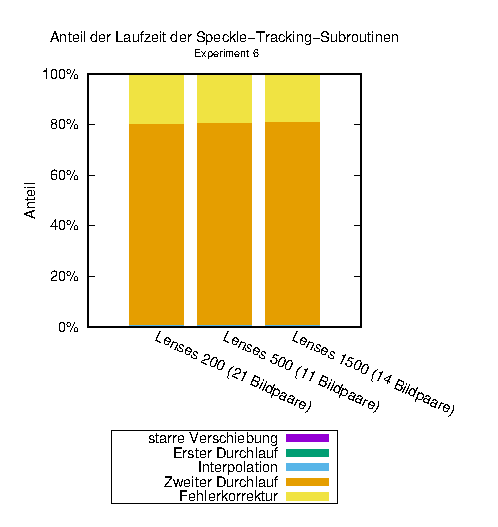
\includegraphics[width=\textwidth]{pdf/speckle_exp6}
			\caption{Experiment 6}
			\label{fig:perc_speckle_exp6}
		\end{subfigure}
		\begin{subfigure}[b]{0.5\textwidth}
			\centering
			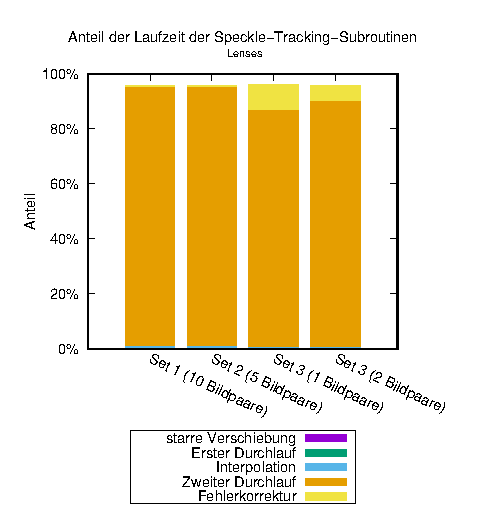
\includegraphics[width=\textwidth]{pdf/speckle_lenses}
			\caption{Lenses}
			\label{fig:perc_speckle_lenses}
		\end{subfigure}
		\caption{Anteile der Laufzeiten des Speckle-Tracking-Algorithmus}
		\label{fig:perc_speckle}
	\end{figure}
\end{center}

Die kumulative Zeit der fünf rechenaufwendigsten Funktionen aller Konfigurationen, dargestellt in Abbildung \ref{fig:perc_slow}, liegt jeweils bei über 95\% der Gesamtzeit. 

\begin{center}
	\begin{figure}[h!]
		\begin{subfigure}[b]{0.5\textwidth}
			\centering
			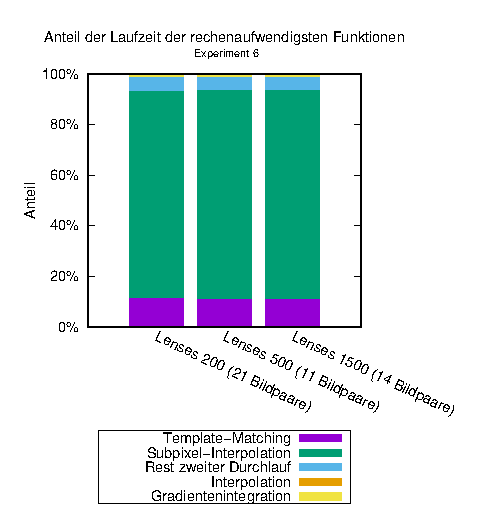
\includegraphics[width=\textwidth]{pdf/slow_exp6}
			\caption{\textit{Experiment 6}}
			\label{fig:perc_slow_exp6}
		\end{subfigure}
		\begin{subfigure}[b]{0.5\textwidth}
			\centering
			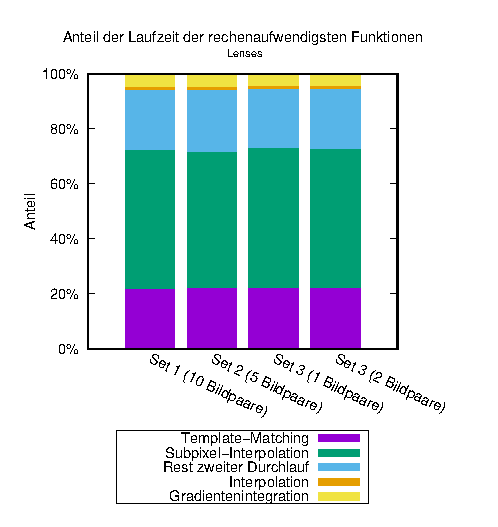
\includegraphics[width=\textwidth]{pdf/slow_lenses}
			\caption{\textit{Lenses}}
			\label{fig:perc_slow_lenses}
		\end{subfigure}
		\caption{Anteile der Laufzeiten der langsamsten Funktionen}
		\label{fig:perc_slow}
	\end{figure}
\end{center}

\section{Performance-Engpässe}

Der Grund der langen Rechenzeiten des Template-Matchings und der Subpixel-Interpolation liegt in der hohen Anzahl der Aufrufe dieser begründet. Der zweite Durchlauf allein wird im \textit{Experiment 6 Lenses 200}-Datensatz über 5.3 Millionen mal aufgerufen. In jedem dieser Aufrufe wird das Template-Matching und die Subpixel-Interpolation jeweils einmal genutzt. Hinzu kommt, dass, bis auf das Temp\-late-Match\-ing, der zweite Durchlauf nur geringen Gebrauch von bereits optimierten Bibliotheken wie numpy macht und somit der Python-Overhead starken Einfluss auf die Laufzeiten hat. Innerhalb des Speckle-Trackings ist der Aufruf des zweiten Durchlaufes mittels der joblib parallelisiert. Diese nutzt standardmäßig die multiprocessing-Bibliothek, welche für jeden Thread einen Fork der gesamten Python-Umgebung erstellen muss \cite{GVB+18}. Die hohe Rechenzeit der Gradienten-Integration ist im Aufruf dieser auf die Größe des Gesamtbildes begründet. Insgesamt hat das Programm eine schlechte CPU-Auslastung von lediglich durchschnittlich 19,635\% \cite{Sch18b}, wodurch häufig einige Kerne nicht oder nur wenig genutzt werden. 

\section{Prüfen der Ergebnisse}

Um die Korrektheit der Ergebnisse nach der Optimierung sicherstellen zu können, wurden die Ergebnisse der Referenzimplementierung unter Eingabe aller Datensätze gespeichert. Diese werden als Referenz für einen bitweisen Abgleich verwendet. Auf Fließkommazahlen basierende Ungenauigkeiten werden hierbei bereits als Fehler gewertet. Nach den initialen Benchmarks wurde diese Methode zur Sicherstellung der Datenintegrität eingesetzt und für geeignet befunden. 